\documentclass[
11pt, % The default document font size, options: 10pt, 11pt, 12pt
%codirector, % Uncomment to add a codirector to the title page
]{charter} 


% El títulos de la memoria, se usa en la carátula y se puede usar el cualquier lugar del documento con el comando \ttitle
\titulo{Actualización Tecnológica de la Organización y Creación de un Modelo de Predicción de Mortalidad como Prueba Piloto} 

% Nombre del posgrado, se usa en la carátula y se puede usar el cualquier lugar del documento con el comando \degreename
\posgrado{Carrera de Especialización en Inteligencia Artificial}

% Tu nombre, se puede usar el cualquier lugar del documento con el comando \authorname
\autor{Ezequiel Scordamaglia} 

% El nombre del director y co-director, se puede usar el cualquier lugar del documento con el comando \supname y \cosupname y \pertesupname y \pertecosupname
\director{Nombre del Director}
\pertenenciaDirector{pertenencia} 
% FIXME:NO IMPLEMENTADO EL CODIRECTOR ni su pertenencia
%\codirector{John Doe} % para que aparezca en la portada se debe descomentar la opción codirector en el documentclass
\pertenenciaCoDirector{FIUBA}

% Nombre del cliente, quien va a aprobar los resultados del proyecto, se puede usar con el comando \clientename y \empclientename
\cliente{Eugenio Bellia}
\empresaCliente{Grupo DUAM}

% Nombre y pertenencia de los jurados, se pueden usar el cualquier lugar del documento con el comando \jurunoname, \jurdosname y \jurtresname y \perteunoname, \pertedosname y \pertetresname.
\juradoUno{Nombre y Apellido (1)}
\pertenenciaJurUno{pertenencia (1)} 
\juradoDos{Nombre y Apellido (2)}
\pertenenciaJurDos{pertenencia (2)}
\juradoTres{Nombre y Apellido (3)}
\pertenenciaJurTres{pertenencia (3)}
 
\fechaINICIO{17 de octubre de 2023}		%Fecha de inicio de la cursada de GdP \fechaInicioName
\fechaFINALPlan{--------COMPLETAR---------} 	%Fecha de final de cursada de GdP
\fechaFINALTrabajo{--------COMPLETAR---------}	%Fecha de defensa pública del trabajo final


\begin{document}

\maketitle
\thispagestyle{empty}
\pagebreak


\thispagestyle{empty}
{\setlength{\parskip}{0pt}
\tableofcontents{}
}
\pagebreak


\section*{Registros de cambios}
\label{sec:registro}


\begin{table}[ht]
\label{tab:registro}
\centering
\begin{tabularx}{\linewidth}{@{}|c|X|c|@{}}
\hline
\rowcolor[HTML]{C0C0C0} 
Revisión & \multicolumn{1}{c|}{\cellcolor[HTML]{C0C0C0}Detalles de los cambios realizados} & Fecha      \\ \hline
0      & Creación del documento                                 &\fechaInicioName \\ \hline
1      & Se completa hasta el punto 4 inclusive                 & 26 de octubre de 2023 \\ \hline
%2      & Se completa hasta el punto 7 inclusive
%		  Se puede agregar algo más \newline
%		  En distintas líneas \newline
%		  Así                                                    & dd/mm/aaaa \\ \hline
%3      & Se completa hasta el punto 11 inclusive                & dd/mm/aaaa \\ \hline
%4      & Se completa el plan	                                 & dd/mm/aaaa \\ \hline
\end{tabularx}
\end{table}

\pagebreak



\section*{Acta de constitución del proyecto}
\label{sec:acta}

\begin{flushright}
Buenos Aires, \fechaInicioName
\end{flushright}

\vspace{2cm}

Por medio de la presente se acuerda con el Lic. \authorname\hspace{1px} que su Trabajo Final de la \degreename\hspace{1px} se titulará ``\ttitle'', y consistirá esencialmente en la incorporación a la organización de nuevas herramientas para el desarrollo de soluciones que utilicen inteligencia artificial y análisis de datos, y que ofrezcan valor agregado a los clientes. Se tomará como prueba piloto el desarrollo de un modelo que prediga el nivel de riego de mortalidad de un paciente en un entorno médico. El mismo tendrá un presupuesto preliminar estimado de 600 h de trabajo y \textcolor{red}{\$1.500.000}, con fecha de inicio \fechaInicioName\hspace{1px} y fecha de presentación pública \fechaFinalName.

Se adjunta a esta acta la planificación inicial.

\vfill

% Esta parte se construye sola con la información que hayan cargado en el preámbulo del documento y no debe modificarla
\begin{table}[ht]
\centering
\begin{tabular}{ccc}
\begin{tabular}[c]{@{}c@{}}Dr. Ing. Ariel Lutenberg \\ Director posgrado FIUBA\end{tabular} & \hspace{2cm} & \begin{tabular}[c]{@{}c@{}}\clientename \\ \empclientename \end{tabular} \vspace{2.5cm} \\ 
\multicolumn{3}{c}{\begin{tabular}[c]{@{}c@{}} \supname \\ Director del Trabajo Final\end{tabular}} \vspace{2.5cm} \\
%\begin{tabular}[c]{@{}c@{}}\jurunoname \\ Jurado del Trabajo Final\end{tabular}     &  & \begin{tabular}[c]{@{}c@{}}\jurdosname\\ Jurado del Trabajo Final\end{tabular}  \vspace{2.5cm}  \\
%\multicolumn{3}{c}{\begin{tabular}[c]{@{}c@{}} \jurtresname\\ Jurado del Trabajo Final\end{tabular}} \vspace{.5cm}                                                                     
\end{tabular}
\end{table}




\section{1. Descripción técnica-conceptual del proyecto a realizar}
\label{sec:descripcion}

Este proyecto, planteado como trabajo final, se realizará para la organización Grupo DUAM en la cual trabajo, donde nos dedicamos a desarrollar software a medida para distintos clientes.
El objetivo principal de este proyecto es incursionar en desarrollos que utilicen las nuevas tecnologías, como son la inteligencia artificial y el análisis de datos, con el fin de proporcionar soluciones innovadoras a problemas preexistentes.
En esta línea, se tomó la decisión de colaborar con uno de nuestros clientes, una empresa médica que opera centros de atención en todo el país, para crear un primer prototipo que haga uso de estas tecnologías y que, al mismo tiempo, les aporte un valor agregado. Por razones de confidencialidad, no podemos revelar la identidad de nuestro cliente. Ellos poseen un sistema de gestión de pacientes donde registran datos médicos asociados a cada paciente, como son estudios médicos, hospitalizaciones, medicamentos prescritos, y muchos otros. Es fundamental en la medicina conocer el estado de salud de los pacientes y evaluar los riesgos asociados a ellos. Esto le permite a los profesionales de la salud ajustar el tratamiento y los medicamentos que  prescriben. Pero predecir los riesgos que puede tener un paciente no es tarea sencilla. La complejidad de las condiciones de salud y la gran cantidad de datos clínicos disponibles hacen extremadamente difícil realizar una predicción de mortalidad de manera manual.
En este contexto, surge la idea de ofrecerles desarrollar un modelo predictivo de mortalidad que pueda aprovechar el poder de la inteligencia artificial y del análisis de datos, para realizar un pronóstico rápido y preciso del nivel de riesgo que tiene un paciente.

En este trabajo, se propone partir por la creación de un modelo predictivo de mortalidad que nos sirva de ejemplo y nos permita ir desarrollando toda la infraestructura necesaria para que el modelo quede disponible para los usuarios. Parte de la infraestructura a desarrollar incluiría la utilización de una plataforma de gestión de modelos y el desarrollo de una interfaz por servicio web. Para el desarrollo de este modelo predictivo puntual, se contará con información de miles de pacientes que fueron atendidos por nuestro cliente y sirven de referencia para el proceso de entrenamiento. Se deberán procesar los datos disponibles, entrenar varios modelos de \textit{machine learning} y \textit{deep learning}, evaluar sus métricas y seleccionar los candidatos que logren los mejores resultados.
El desarrollo de este tipo de modelos predictivos, administrados por una plataforma de gestión integral y accesibles por servicio web, nos permitirá adentrarnos en un mercado en constante evolución que demanda soluciones innovadoras. En la Figura \ref{fig:diagBloques} se muestra un diagrama de la solución propuesta para resolver el caso piloto.

\begin{figure}[htpb]
\centering 
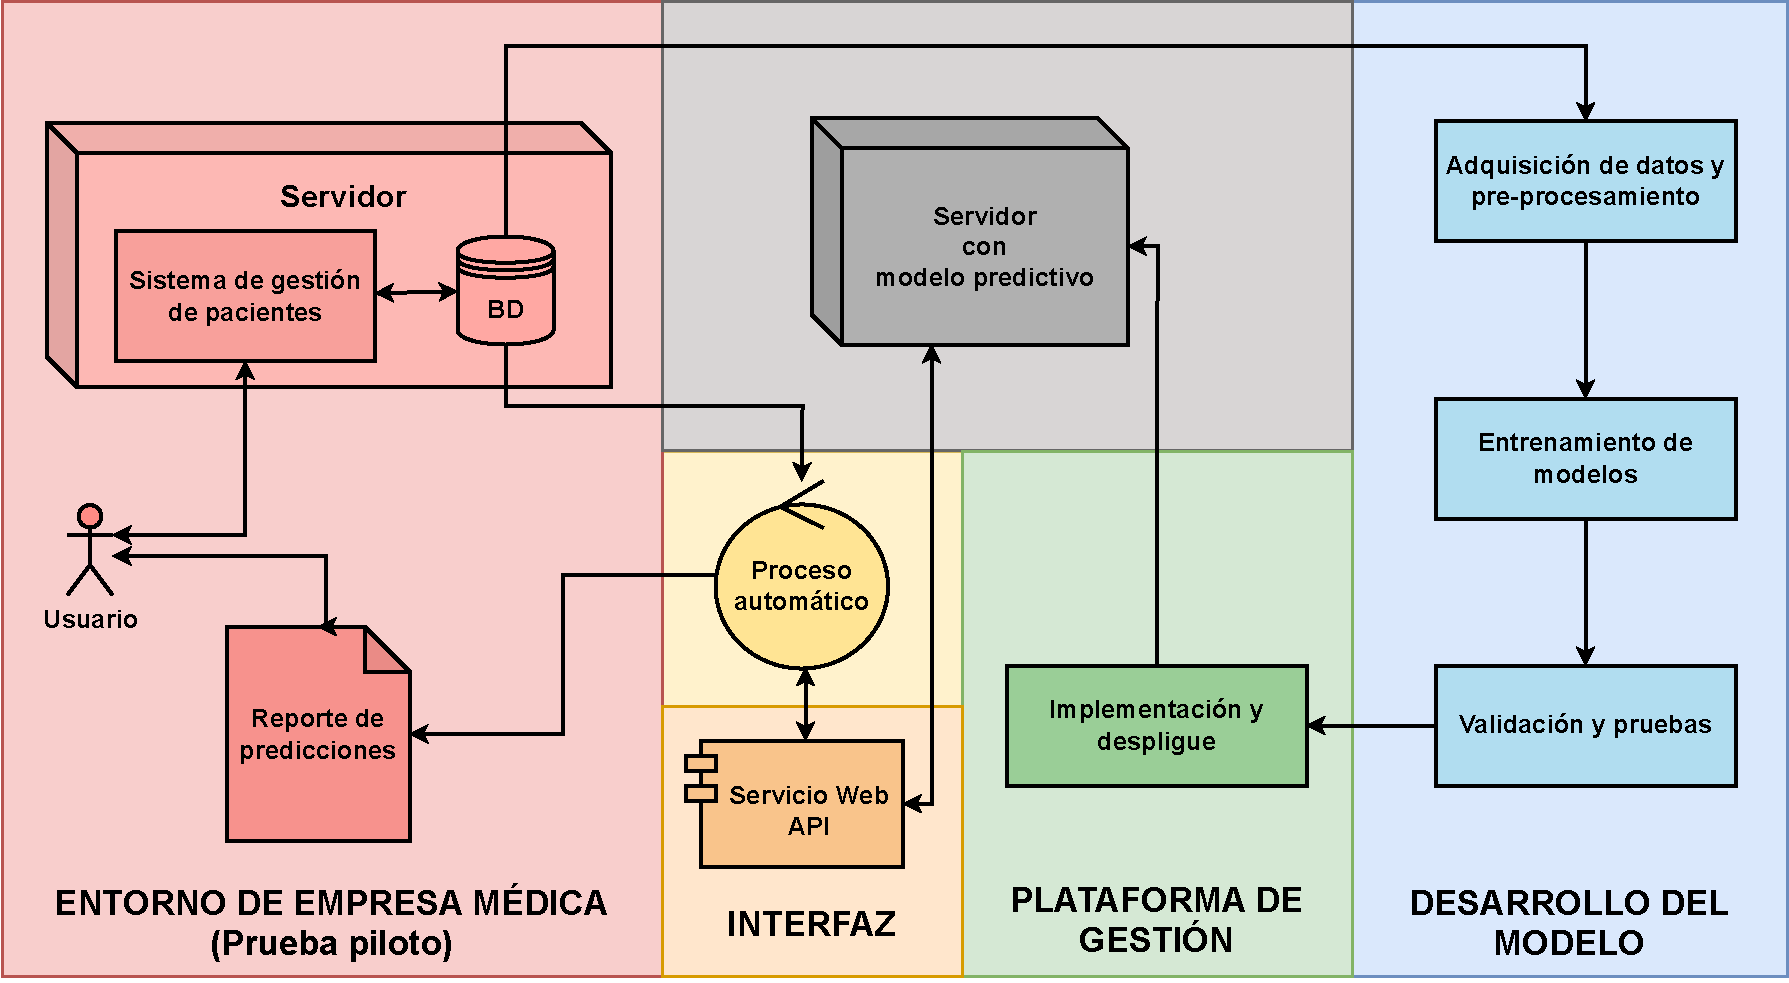
\includegraphics[width=.6\textwidth]{./Figuras/DiagramaDeBloques.pdf}
\caption{Diagrama en bloques del sistema}
\label{fig:diagBloques}
\end{figure}

Si bien parte del proyecto se limitará a dar solución a un problema puntual en el ámbito médico, el objetivo final es poder brindar soluciones a distintos clientes, incorporando los beneficios de las nuevas tecnologías.
El uso de la inteligencia artificial y el análisis de datos está en auge actualmente, y muchas industrias de distintos campos ya están logrando resultados exitosos. En la medicina ya se han utilizado para la predicción del desarrollo de enfermedades como la diabetes o el cáncer, y también para detectar formas extrañas en imágenes. 
Esto se debe a que los modelos utilizados tienen la capacidad de reconocer patrones en grandes conjuntos de datos.
Para poder generar predicciones es necesario utilizar datos históricos en el entrenamiento, donde los modelos descubren relaciones entre ellos. Luego, por métodos estadísticos, logran predecir eventos futuros basados en dichas relaciones.
Dado que ya se cuenta con los datos históricos de miles de pacientes, este tipo de tecnología podría servir perfectamente para resolver la problemática actual de nuestro cliente. 
El desarrollo de este proyecto tendría dos resultados importantes: dotar a nuestra organización de los conocimientos y herramientas necesarias para resolver problemas que requieran el uso de las nuevas tecnologías, y obtener un producto que resuelva una problemática real, ayudando al personal médico a guiar su trabajo sobre los pacientes más críticos y, en última instancia, salvar vidas.

\section{2. Identificación y análisis de los interesados}
\label{sec:interesados}

\begin{table}[ht]
%\caption{Identificación de los interesados}
%\label{tab:interesados}
\begin{tabularx}{\linewidth}{@{}|l|X|X|l|@{}}
\hline
\rowcolor[HTML]{C0C0C0} 
Rol           & Nombre y Apellido & Organización   & Puesto        \\ \hline
Cliente       & \clientename      & \empclientename & Director      \\ \hline
Responsable   & \authorname       & FIUBA           & Alumno        \\ \hline
Colaboradores & \parbox{4.1cm}{Colaborador confidencial \\ Colaborador confidencial}  & \parbox{4.2cm}{Organización confidencial \\ Organización confidencial} & \parbox{4.2cm}{Gerente de Sistemas \\ Asesor de Presidencia} \\ \hline
Orientador    & \supname          & \pertesupname    & Director Trabajo final \\ \hline
Usuario final & Personal Médico   & Organización confidencial  & Usuario del sistema   \\ \hline
\end{tabularx}
\end{table}

\begin{itemize}
	\item Cliente: Está a favor del desarrollo de este proyecto para impulsar la organización a nuevos mercados y/o ofrecerle desarrollos innovadores a los clientes actuales.
	\item Colaboradores: El Asesor de presidencia no tiene mucho tiempo para dedicarle al proyecto, pero puede aportar conocimientos médicos para seleccionar las características mas importantes que tengan relación con la mortalidad de los pacientes. Está a favor del desarrollo del proyecto y aportará lo que sea necesario. El Gerente de Sistemas tampoco tiene mucho tiempo para dedicarle al proyecto, pero es quien nos dará permiso para la utilización de los datos. Como no solicitó el desarrollo del proyecto puede que demore en responder o en tomar decisiones cuando se realice la integración.
	\item Orientador: Puede ayudar mucho en el tratamiento de los datos antes de entrenar los modelos.
	\item Usuario final: Necesitará que la predicciones que realiza el modelo estén disponibles en todo momento.
\end{itemize}


\section{3. Propósito del proyecto}
\label{sec:proposito}

El propósito principal de este proyecto es dotar a nuestra organización de nuevas herramientas y capacidades en el ámbito de la inteligencia artificial y el análisis de datos, para poder ofrecer soluciones innovadoras a clientes nuevos o existentes, y poder insertarnos en un mercado que se encuentra en constante crecimiento. 

\section{4. Alcance del proyecto}
\label{sec:alcance}

El presente proyecto incluye principalmente la instalación y configuración de una plataforma de gestión de modelos, que permita administrar versiones y ejecutar acciones como el despliegue y el re-entrenamiento de modelos.
Como prueba piloto, se desarrollará un modelo de predicción de mortalidad, que se incorporará a la plataforma de gestión, y también una interfaz que actúe como nexo entre el modelo predictivo y el usuario final.
Para el desarrollo del modelo, se realizarán las tareas de extracción de los datos, su procesamiento, el entrenamiento de los modelos y la evaluación de sus métricas. 
Una vez que se cuente con un modelo entrenado, se realizarán las tareas referidas al despliegue del modelo. 
Con el fin de automatizar la llamada al modelo, se desarrollará también un proceso que envíe automáticamente pedidos de predicciones de todos los pacientes activos cada cierto tiempo al modelo, para que el usuario final cuente con un reporte actualizado en todo momento.
El resultado del modelo podrá ser binario (hay riesgo o no hay riesgo), o categórico, devolviendo un grado de riesgo para ese paciente. Esto se definirá luego de realizar un análisis de los datos disponibles y de los modelos seleccionados para el entrenamiento.

El presente proyecto no incluye el desarrollo de una plataforma de gestión, sino que se elegirá una existente que cumpla con los requerimientos del proyecto. No se desarrollará una interfaz web orientada al usuario final, sino que se desarrollará un servicio web que sea utilizado por procesos automáticos. No se incluirán procesos que disparen el re-entrenamiento automático ante cambios en los datos. El re-entrenamiento del modelo se realizará manualmente por un operador cuando sea necesario.
No se incluye la instalación del modelo predictivo en el entorno productivo de nuestro cliente, sino que para el proyecto presentado para este posgrado, se trabajará en un entorno propio de Grupo DUAM que incluirá la plataforma de gestión de modelos, el modelo predictivo y la interfaz por servicio web. Lo único que se instalará en el entorno del cliente será el proceso que recupere datos de los pacientes y llame al servicio web cada cierto período de tiempo para recuperar las predicciones. Esto debe aclararse ya que la instalación de toda la infraestructura en el entorno del cliente no es el objetivo principal de este proyecto, y podría dejarse a cargo del equipo de sistemas del cliente.

\section{5. Supuestos del proyecto}
\label{sec:supuestos}

Para el desarrollo del presente proyecto se supone que:

\begin{itemize}
	\item Se dispone de tiempo en horario laboral para avanzar en el proyecto.
	\item Se dispone de los equipos necesarios para realizar el procesamiento de los datos y el entrenamiento de los modelos.
	\item Se dispone de un ambiente donde poder instalar y configurar la plataforma de gestión, disponibilizar la interfaz por web service y desplegar el modelo para realizar predicciones. 
	\item No hay urgencia en el desarrollo del modelo predictivo.		
	\item Se tiene acceso a los datos médicos de los pacientes.
	\item Se cuenta con un conjunto inicial de datos lo suficientemente grande y representativo para entrenar los modelos de inteligencia artificial de manera efectiva.
	\item Se cuenta con el apoyo de un responsable médico que dé soporte en la selección de variables médicas a utilizar en el entrenamiento de los modelos y también en la interpretación clínica de las predicciones realizadas.
	\item Se mantendrá la protección de datos sensibles de los pacientes y de nuestro cliente en todo momento.		
\end{itemize}

\section{6. Requerimientos}
\label{sec:requerimientos}

\begin{consigna}{red}

\begin{enumerate}
	\item Requerimientos funcionales
		\begin{enumerate}
			\item La plataforma de gestión de modelos deberá permitir desplegar modelos en diversos ambientes y disparar un proceso manual de re-entrenamiento cuando sea necesario.
			\item La interfaz por servicio web deberá recibir datos médicos de uno o varios pacientes y devolver las predicciones asociadas a ellos.			
			\item El modelo predictivo deberá tener una precisión de al menos un 75\%.
			\item El proceso que solicita predicciones y genera el reporte al usuario deberá poder ejecutarse automáticamente cada cierto período de tiempo.		
			\item Las predicciones individuales que realice el modelo deberán generarse en cuestión de segundos.
			\item El modelo	deberá estar disponible en todo momento.
			\item Durante el entrenamiento del modelo se deberá resguardar la confidencialidad de los datos de los pacientes.
			\item El reporte de predicciones que le llegue al usuario final deberá tener un formato claro y comprensible.
		\end{enumerate}
	\item Requerimientos de documentación
		\begin{enumerate}
			\item La documentación de la interfaz por servicio web deberá incluir la lista de métodos disponibles con su detalle.
			\item La documentación del modelo predictivo deberá incluir el lenguaje de programación con el que se desarrolló, las librerías utilizadas, una descripción del procesamiento realizado sobre los datos recibidos y los modelos que se compararon en la etapa de desarrollo.
		\end{enumerate}
\end{enumerate}

\end{consigna}

\section{7. Historias de usuarios (\textit{Product backlog})}
\label{sec:backlog}

\begin{consigna}{red}

Se describirán una serie de historias de usuario clasificadas con un puntaje que va del 1 al 5 e indican la importancia que tienen a nivel global en el contexto de este proyecto.

Como director de la empresa Grupo DUAM quiero contar con un ambiente en el cual se puedan incluir nuevos modelos predictivos que resuelvan las problemáticas de mis clientes y un equipo capacitado para responder a esa demanda. (5)

Como personal médico de la empresa cliente que colabora en la creación del modelo predictivo, quiero contar con un reporte de predicciones de riesgos de mortalidad de todos los pacientes de mi centro, para poder realizar ajustes en los tratamientos y medicaciones prescritas. (4)

Como director medico nacional de la empresa cliente que colabora en la creación del modelo predictivo, quiero contar con un reporte de predicciones de riesgos de mortalidad de todos los pacientes de la red, para realizar estadísticas y comparaciones entre los centros, aplicando directivas para mejorar la situación en cada uno. (3)

\end{consigna}

\section{8. Entregables principales del proyecto}
\label{sec:entregables}

\begin{consigna}{red}

Los entregables del proyecto son (ejemplo):

\begin{itemize}
	\item Documentación del servicio web
	\item Documentación del modelo predictivo 
	\item Modelo predictivo de mortalidad
	\item Plataforma de gestión de modelos correctamente configurada
	\item Interfaz por web servicie	
	\item Proceso que solicite predicciones y arme un reporte para el usuario de forma automática.
	\item Informe final
\end{itemize}

\end{consigna}

\section{9. Desglose del trabajo en tareas}
\label{sec:wbs}

\begin{consigna}{red}
El WBS debe tener relación directa o indirecta con los requerimientos.  Son todas las actividades que se harán en el proyecto para dar cumplimiento a los requerimientos. Se recomienda mostrar el WBS mediante una lista indexada:

\begin{enumerate}
\item Grupo de tareas 1
	\begin{enumerate}
	\item Tarea 1 (tantas h)
	\item Tarea 2 (tantas hs)
	\item Tarea 3 (tantas h)
	\end{enumerate}
\item Grupo de tareas 2
	\begin{enumerate}
	\item Tarea 1 (tantas h)
	\item Tarea 2 (tantas h)
	\item Tarea 3 (tantas h)
	\end{enumerate}
\item Grupo de tareas 3
	\begin{enumerate}
	\item Tarea 1 (tantas h)
	\item Tarea 2 (tantas h)
	\item Tarea 3 (tantas h)
	\item Tarea 4 (tantas h)
	\item Tarea 5 (tantas h)
	\end{enumerate}
\end{enumerate}

Cantidad total de horas: (tantas h)

Se recomienda que no haya ninguna tarea que lleve más de 40 h. 

\end{consigna}

\section{10. Diagrama de Activity On Node}
\label{sec:AoN}

\begin{consigna}{red}
Armar el AoN a partir del WBS definido en la etapa anterior. 

%La figura \ref{fig:AoN} fue elaborada con el paquete latex tikz y pueden consultar la siguiente referencia \textit{online}:

%\url{https://www.overleaf.com/learn/latex/LaTeX_Graphics_using_TikZ:_A_Tutorial_for_Beginners_(Part_3)\%E2\%80\%94Creating_Flowcharts}

\end{consigna}

\begin{figure}[htpb]
\centering 
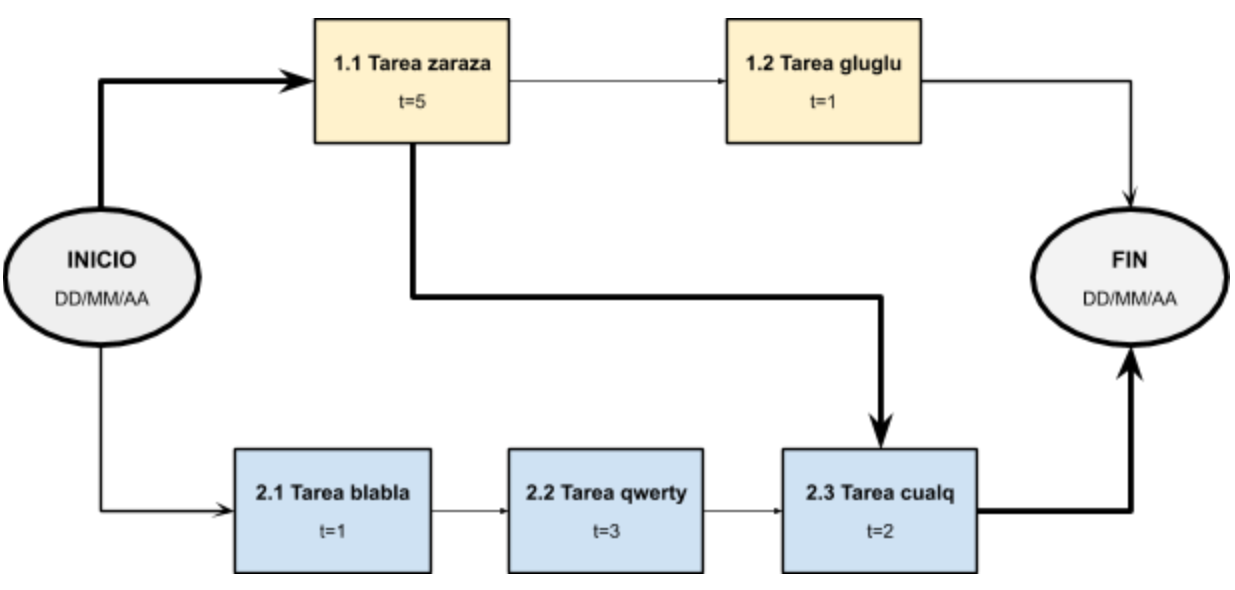
\includegraphics[width=.8\textwidth]{./Figuras/AoN.png}
\caption{Diagrama de \textit{Activity on Node}.}
\label{fig:AoN}
\end{figure}

Indicar claramente en qué unidades están expresados los tiempos.
De ser necesario indicar los caminos semicríticos y analizar sus tiempos mediante un cuadro.
Es recomendable usar colores y un cuadro indicativo describiendo qué representa cada color, como se muestra en el siguiente ejemplo:



\section{11. Diagrama de Gantt}
\label{sec:gantt}

\begin{consigna}{red}

Existen muchos programas y recursos \textit{online} para hacer diagramas de Gantt, entre los cuales destacamos:

\begin{itemize}
\item Planner
\item GanttProject
\item Trello + \textit{plugins}. En el siguiente link hay un tutorial oficial: \\ \url{https://blog.trello.com/es/diagrama-de-gantt-de-un-proyecto}
\item Creately, herramienta online colaborativa. \\\url{https://creately.com/diagram/example/ieb3p3ml/LaTeX}
\item Se puede hacer en latex con el paquete \textit{pgfgantt}\\ \url{http://ctan.dcc.uchile.cl/graphics/pgf/contrib/pgfgantt/pgfgantt.pdf}
\end{itemize}

Pegar acá una captura de pantalla del diagrama de Gantt, cuidando que la letra sea suficientemente grande como para ser legible. 
Si el diagrama queda demasiado ancho, se puede pegar primero la ``tabla'' del Gantt y luego pegar la parte del diagrama de barras del diagrama de Gantt.

Configurar el software para que en la parte de la tabla muestre los códigos del EDT (WBS).\\
Configurar el software para que al lado de cada barra muestre el nombre de cada tarea.\\
Revisar que la fecha de finalización coincida con lo indicado en el Acta Constitutiva.

En la figura \ref{fig:gantt}, se muestra un ejemplo de diagrama de Gantt realizado con el paquete de \textit{pgfgantt}. En la plantilla pueden ver el código que lo genera y usarlo de base para construir el propio.

\begin{figure}[htbp]
\begin{center}
\begin{ganttchart}{1}{12}
  \gantttitle{2020}{12} \\
  \gantttitlelist{1,...,12}{1} \\
  \ganttgroup{Group 1}{1}{7} \\
  \ganttbar{Task 1}{1}{2} \\
  \ganttlinkedbar{Task 2}{3}{7} \ganttnewline
  \ganttmilestone{Milestone o hito}{7} \ganttnewline
  \ganttbar{Final Task}{8}{12}
  \ganttlink{elem2}{elem3}
  \ganttlink{elem3}{elem4}
\end{ganttchart}
\end{center}
\caption{Diagrama de Gantt de ejemplo}
\label{fig:gantt}
\end{figure}


\begin{landscape}
\begin{figure}[htpb]
\centering 
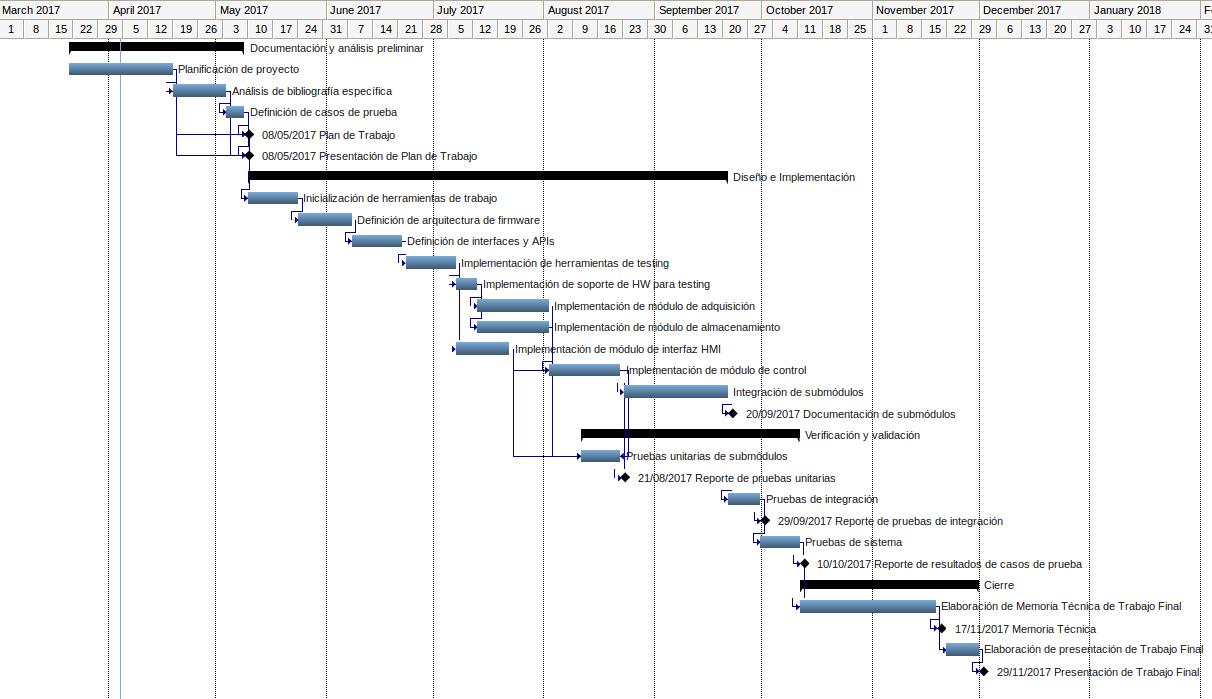
\includegraphics[height=.85\textheight]{./Figuras/Gantt-2.png}
\caption{Ejemplo de diagrama de Gantt rotado}
\label{fig:diagGantt}
\end{figure}

\end{landscape}

\end{consigna}


\section{12. Presupuesto detallado del proyecto}
\label{sec:presupuesto}

\begin{consigna}{red}
Si el proyecto es complejo entonces separarlo en partes:
\begin{itemize}
	\item Un total global, indicando el subtotal acumulado por cada una de las áreas.
	\item El desglose detallado del subtotal de cada una de las áreas.
\end{itemize}

IMPORTANTE: No olvidarse de considerar los COSTOS INDIRECTOS.

\end{consigna}

\begin{table}[htpb]
\centering
\begin{tabularx}{\linewidth}{@{}|X|c|r|r|@{}}
\hline
\rowcolor[HTML]{C0C0C0} 
\multicolumn{4}{|c|}{\cellcolor[HTML]{C0C0C0}COSTOS DIRECTOS} \\ \hline
\rowcolor[HTML]{C0C0C0} 
Descripción &
  \multicolumn{1}{c|}{\cellcolor[HTML]{C0C0C0}Cantidad} &
  \multicolumn{1}{c|}{\cellcolor[HTML]{C0C0C0}Valor unitario} &
  \multicolumn{1}{c|}{\cellcolor[HTML]{C0C0C0}Valor total} \\ \hline
 &
  \multicolumn{1}{c|}{} &
  \multicolumn{1}{c|}{} &
  \multicolumn{1}{c|}{} \\ \hline
 &
  \multicolumn{1}{c|}{} &
  \multicolumn{1}{c|}{} &
  \multicolumn{1}{c|}{} \\ \hline
\multicolumn{1}{|l|}{} &
   &
   &
   \\ \hline
\multicolumn{1}{|l|}{} &
   &
   &
   \\ \hline
\multicolumn{3}{|c|}{SUBTOTAL} &
  \multicolumn{1}{c|}{} \\ \hline
\rowcolor[HTML]{C0C0C0} 
\multicolumn{4}{|c|}{\cellcolor[HTML]{C0C0C0}COSTOS INDIRECTOS} \\ \hline
\rowcolor[HTML]{C0C0C0} 
Descripción &
  \multicolumn{1}{c|}{\cellcolor[HTML]{C0C0C0}Cantidad} &
  \multicolumn{1}{c|}{\cellcolor[HTML]{C0C0C0}Valor unitario} &
  \multicolumn{1}{c|}{\cellcolor[HTML]{C0C0C0}Valor total} \\ \hline
\multicolumn{1}{|l|}{} &
   &
   &
   \\ \hline
\multicolumn{1}{|l|}{} &
   &
   &
   \\ \hline
\multicolumn{1}{|l|}{} &
   &
   &
   \\ \hline
\multicolumn{3}{|c|}{SUBTOTAL} &
  \multicolumn{1}{c|}{} \\ \hline
\rowcolor[HTML]{C0C0C0}
\multicolumn{3}{|c|}{TOTAL} &
   \\ \hline
\end{tabularx}%
\end{table}


\section{13. Gestión de riesgos}
\label{sec:riesgos}

\begin{consigna}{red}
a) Identificación de los riesgos (al menos cinco) y estimación de sus consecuencias:
 
Riesgo 1: detallar el riesgo (riesgo es algo que si ocurre altera los planes previstos de forma negativa)
\begin{itemize}
	\item Severidad (S): mientras más severo, más alto es el número (usar números del 1 al 10).\\
	Justificar el motivo por el cual se asigna determinado número de severidad (S).
	\item Probabilidad de ocurrencia (O): mientras más probable, más alto es el número (usar del 1 al 10).\\
	Justificar el motivo por el cual se asigna determinado número de (O). 
\end{itemize}   

Riesgo 2:
\begin{itemize}
	\item Severidad (S): 
	\item Ocurrencia (O):
\end{itemize}

Riesgo 3:
\begin{itemize}
	\item Severidad (S): 
	\item Ocurrencia (O):
\end{itemize}


b) Tabla de gestión de riesgos:      (El RPN se calcula como RPN=SxO)

\begin{table}[htpb]
\centering
\begin{tabularx}{\linewidth}{@{}|X|c|c|c|c|c|c|@{}}
\hline
\rowcolor[HTML]{C0C0C0} 
Riesgo & S & O & RPN & S* & O* & RPN* \\ \hline
       &   &   &     &    &    &      \\ \hline
       &   &   &     &    &    &      \\ \hline
       &   &   &     &    &    &      \\ \hline
       &   &   &     &    &    &      \\ \hline
       &   &   &     &    &    &      \\ \hline
\end{tabularx}%
\end{table}

Criterio adoptado: 
Se tomarán medidas de mitigación en los riesgos cuyos números de RPN sean mayores a...

Nota: los valores marcados con (*) en la tabla corresponden luego de haber aplicado la mitigación.

c) Plan de mitigación de los riesgos que originalmente excedían el RPN máximo establecido:
 
Riesgo 1: plan de mitigación (si por el RPN fuera necesario elaborar un plan de mitigación).
  Nueva asignación de S y O, con su respectiva justificación:
  - Severidad (S): mientras más severo, más alto es el número (usar números del 1 al 10).
          Justificar el motivo por el cual se asigna determinado número de severidad (S).
  - Probabilidad de ocurrencia (O): mientras más probable, más alto es el número (usar del 1 al 10).
          Justificar el motivo por el cual se asigna determinado número de (O).

Riesgo 2: plan de mitigación (si por el RPN fuera necesario elaborar un plan de mitigación).
 
Riesgo 3: plan de mitigación (si por el RPN fuera necesario elaborar un plan de mitigación).

\end{consigna}


\section{14. Gestión de la calidad}
\label{sec:calidad}

\begin{consigna}{red}
Elija al menos diez requerientos que a su criterio sean los más importantes/críticos/que aportan más valor y para cada uno de ellos indique las acciones de verificación y validación que permitan asegurar su cumplimiento.

\begin{itemize} 
\item Req \#1: copiar acá el requerimiento.

\begin{itemize}
	\item Verificación para confirmar si se cumplió con lo requerido antes de mostrar el sistema al cliente. Detallar 
	\item Validación con el cliente para confirmar que está de acuerdo en que se cumplió con lo requerido. Detallar  
\end{itemize}

\end{itemize}

Tener en cuenta que en este contexto se pueden mencionar simulaciones, cálculos, revisión de hojas de datos, consulta con expertos, mediciones, etc.  Las acciones de verificación suelen considerar al entregable como ``caja blanca'', es decir se conoce en profundidad su funcionamiento interno.  En cambio, las acciones de validación suelen considerar al entregable como ``caja negra'', es decir, que no se conocen los detalles de su funcionamiento interno.

\end{consigna}

\section{15. Procesos de cierre}    
\label{sec:cierre}

\begin{consigna}{red}
Establecer las pautas de trabajo para realizar una reunión final de evaluación del proyecto, tal que contemple las siguientes actividades:

\begin{itemize}
	\item Pautas de trabajo que se seguirán para analizar si se respetó el Plan de Proyecto original:
	 - Indicar quién se ocupará de hacer esto y cuál será el procedimiento a aplicar. 
	\item Identificación de las técnicas y procedimientos útiles e inútiles que se emplearon, y los problemas que surgieron y cómo se solucionaron:
	 - Indicar quién se ocupará de hacer esto y cuál será el procedimiento para dejar registro.
	\item Indicar quién organizará el acto de agradecimiento a todos los interesados, y en especial al equipo de trabajo y colaboradores:
	  - Indicar esto y quién financiará los gastos correspondientes.
\end{itemize}

\end{consigna}


\end{document}
